\chapter{Second Sprint}\label{chap:sprint2}
We chose to work with \launcher during the second sprint as well.\vagner{Skal vi muligvis sige noget om at vi arbejde med launcher igennem hele projektet, frem for at bare sige det hver gang vi kommer til en Sprint start?}
Having completed all remaining task from the first sprint, the second is upon making a foundation for future work.
The idea of making a settings button in \launcher is explored by the means of prototypes and customer meetings.\vagner{hvor var det vi fik ideen med settings in the first place?}
The goal for the sprint is to have specifications for the settings.

\section{Sprint Overview}\label{sec:sprint2:overview}
As the described in \cref{sec:sprint1:review}, the end of the first sprint left us unsure of whether there was more work to be done on \launcher, and if so, what this work could be. 
We decide that it is necessary to arrange a meeting with some of the clients, in part to hear their thoughts on the current version of \launcher, and in part to discover new features.
During the first sprint we informally discussed ideas for new features.
These features include an improved format for the profile selector, and a new Settings application, providing a uniform interface for changing settings across all applications. 
To provide a good foundation for presenting and discussing these ideas with the customers, we design a number of prototype drawings of how our ideas could be realized.

A separate important issue in this sprint is adapting \launcher for new versions its dependencies. 
The \textit{OasisLib} library underwent drastic changes at the end of the first sprint, which unfortunately resulted in several applications, including \launcher, being unable to run.

In summary, the main points of this sprint are:

\begin{itemize}
\item Description of the designed prototypes in \cref{sec:sprint2:analysis}, with summaries of the first meeting in \cref{sec:sprint2:firstmeeting} and the second meeting in \cref{sec:sprint2:secondmeeting}.
\item Description of the migration to the new OasisLib in \cref{sec:sprint2:developments}
\end{itemize}\vagner{Is this seriously all we did?}

\section{Analysis and Design}\label{sec:sprint2:analysis}
Intro here...
\subsection{Prototypes}\label{sec:sprint2:prototypes}

At the end of first sprint, the existing features of \launcher were polished and the project would only need to be kept updated with the implementation of the database. \vagner{Verify that this is indeed what actually happened}
However, the review meeting of sprint one determined that it was desired for launcher to possibly have additional features:

\begin{itemize}
\item Selection of profiles might be desired to be selectable elsewhere in \launcher without starting an application.
\item Settings for different applications could be set from an activity accessed from \launcher.
\item Specification of which applications different users can access could likewise be set from and accessed from \launcher.
\end{itemize}

It was decided to have a brainstorm to gather ideas regarding these features, create prototypes of the best ones\footnote{The prototypes regarded as being the best, were deemed so by the project group.} and present these to the customers for feedback.

The prototypes created were \textbf{low fidelity, horizontal} prototypes, as described in \citet[p. 184-195]{debBook}, made partly with screenshots of existing functionality and partly with the modelling tool Gliffy (\citet{gliffy}).
The purpose was to convey several different ways of including the above features, while not spending too much time creating them.

\subsubsection{Profile Selection}

At the end of sprint one, the profile selection would only appear when launching an application, as illustrated by the state chart diagram in \Cref{fig:statechartProfileSelectorInitial}.
\insertfigure{width=\textwidth}{statechartProfileSelectorInitial}{State chart diagram for the original process of choosing a profile.}{fig:statechartProfileSelectorInitial}
Two alternatives where suggested:
\begin{itemize}
\item Selection of a different profile from within \launcher.
This would work by pressing the profile picture, giving a list of profiles to choose from.
Being relevant only for a guardian, the profiles selectable should only be the guardian itself and the child related to him or her.

\item Selection of a different profile from within each individual application.
While this solution does not require any modification of \launcher, it was a favourable option.
Each application would then have its own profile selection button to initiate the activities
\end{itemize}

Common for both alternatives was to display the currently selected profile in the top of the pane.
Illustrations can be seen on \Cref{fig:profileselectionlauncherdropdown,fig:profileselectionapppopup} respectively. For an explanation of the suggested process of choosing a profile see the state chart diagram in \Cref{fig:statechartProfileSelectorBubble}.

\begin{figure}[h] % Billeder af profile selector
\centering
    \begin{subfigure}[t]{.48\textwidth}
    \centering
    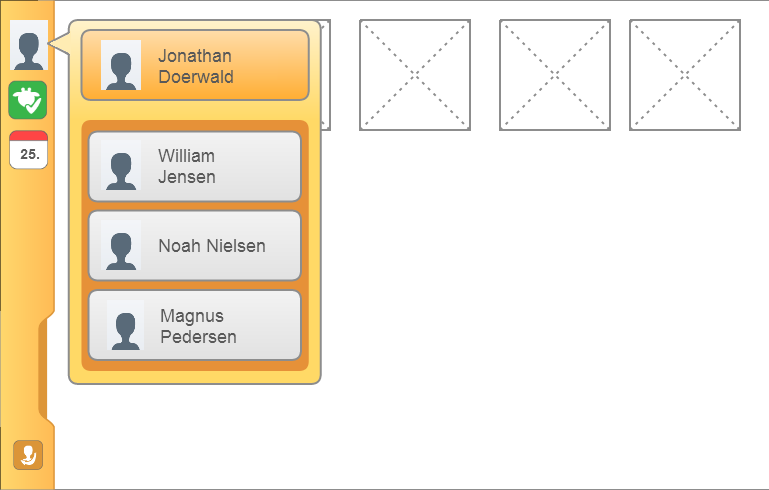
\includegraphics[width=\textwidth]{sprint2/profileselectionhomescreen-dropdown}
    \caption{The dropdown profile selection option. This would appear when tapping ones profile picture as a guardian.}
    \label{fig:profileselectionlauncherdropdown}
    \end{subfigure}
    \hfill
    \begin{subfigure}[t]{.48\textwidth}
    \centering
    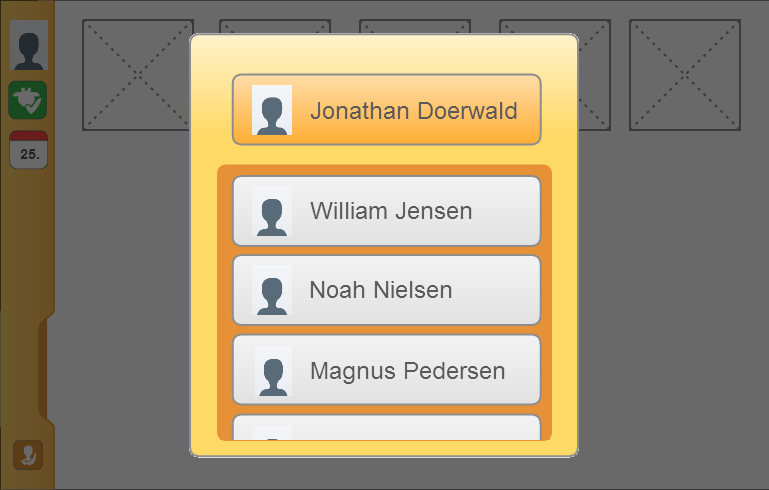
\includegraphics[width=\textwidth]{sprint2/profileselection-dialog-finish}
    \caption{The profile selection pop up. These would only appear while pressing the appropriate button while inside an application.}
    \label{fig:profileselectionapppopup}
    \end{subfigure}\\
    \begin{center}
    \begin{subfigure}[t]{1\textwidth}
    \includegraphics[width=\textwidth]{figures/statechartProfileSelectorBubble.tikz}
    \caption{State chart diagram for the suggested alternative process of choosing a profile.}
    \label{fig:statechartProfileSelectorBubble}
    \end{subfigure}
    \end{center}

\caption{Suggestions for the new profile selector.}
\label{fig:drawerstates}
\end{figure}

\subsubsection{Settings}

At the end of first sprint, settings for different applications where handled inside those applications exclusively.
The idea of centralizing the settings for the different applications was formed both to streamline data for the database, but also to grant the user a better overview over the settings shared by applications.

Again, two alternatives were presented:
\begin{itemize}
\item A settings activity, accessible from \launcher only.
This activity would contain settings for all applications enabled for the selected user, as well as selecting which applications should be enabled for that profile.
This would also include the native Android settings.
\item Letting each application have a settings button.
This would preserve the current setup.
\end{itemize}

The first option is the most encompassing one, containing functionality for both manipulate settings for other applications and decide which applications can be used with different users.
It was furthermore discussed to add functionality, allowing the user to add applications from Google Play to \launcher.
The settings part of the settings activity can be seen in \Cref{fig:settingsprototype}, while the application management part can be seen in \Cref{fig:appsmanagement}.

The second option is more centred on making the settings screen streamlined across applications and would thus be a operative project with the GUI project group.
An example of settings for \launcher can be seen in \Cref{fig:appsettingsprototype}.

\begin{figure}[h] % Billeder af draweren i �ben og lukket tilstand
\centering
    \begin{subfigure}[t]{.48\textwidth}
    \centering
    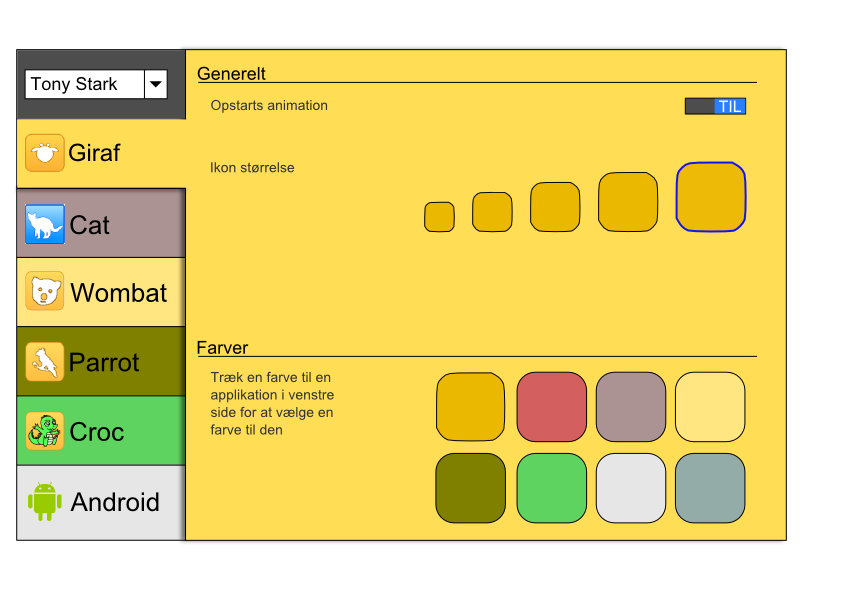
\includegraphics[width=\textwidth]{sprint2/settings}
    \caption{The settings manipulation part of the settings application. in this example, settings for \launcher can be seen. The current profile being edited can be seen in the top left corner.}
    \label{fig:settingsprototype}
    \end{subfigure}
    \hfill
    \begin{subfigure}[t]{.48\textwidth}
    \centering
    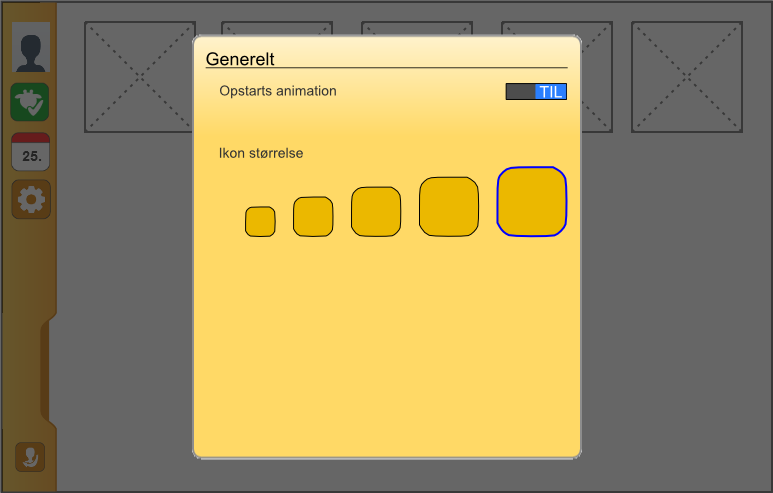
\includegraphics[width=\textwidth]{sprint2/settings-dialog}
    \caption{The settings for a single application. In this example, the settings for \launcher can be seen.}
    \label{fig:appsettingsprototype}
    \end{subfigure}\\
    \begin{subfigure}[t]{.48\textwidth}
    \centering
    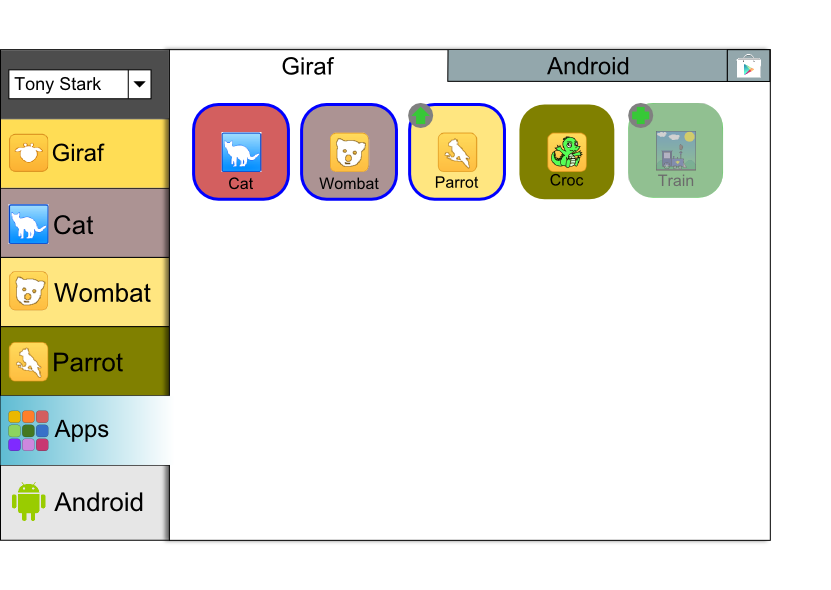
\includegraphics[width=\textwidth]{sprint2/apps-colorexperiment}
    \caption{The application management part of the settings application. \giraf or Android (Google Play) applications can be chosen in the pane in the top. The current profile being edited can be seen in the top left corner.}
    \label{fig:appsmanagement}
    \end{subfigure}
\caption{Suggestions for settings and application management.}
\label{fig:drawerstates}
\end{figure}

\subsubsection{Profile Info}
\frederik{Maaske vi skal undlade denne section, kunderne var ikke vilde med det.}
The group had an idea of displaying information about the user currently logged in in the drawer section of \launcher.
This is a relatively small feature that would be trivial to implement.
An example can be seen in \Cref{fig:profileinfo}.

\insertfigure{width=0.48\textwidth}{sprint2/profil-info}{An example of information about a user seen in the drawer.}{fig:profileinfo}
\section{First Customer Meeting}\label{sec:sprint2:firstmeeting}
This section focuses on the first customer meeting that was held to determine the viability of the thoughts described in \cref{sec:sprint2:prototypes}.

It was held together with one customer and an external contact on the 1st of April, 2014.
The customer is Drazenko Banjak from the institution called Egebakken, which is a school for children with autism.
The external contact is Pernille Hansen Krogh, the owner of a company called Mymo, which works with design and decor optimized for learning.\footnote{In plural they are referred to as \textit{customers}.}


\subsection{Feedback}\label{sec:firstmeeting:feedback}
Since the contents of the meeting mostly concerned new developments, a slide show was made to support the presentation of the prototypes.
Following that the customers not staying to discuss \giraf at the status meeting, a tablet with the most recent version of \launcher was also brought to get feedback on the changes made during the first sprint (\cref{chap:sprint1}).


\subsubsection{Profile Selector}
The profile selector prototypes (\cref{fig:profileselectionlauncherdropdown,fig:profileselectionapppopup}) was presented, and both customers were thrilled about the idea of being able to easily switch profiles from \launcher and each \giraf application individually.
The design was by Pernille considered as being ``clean and intuitive'', as outlined in \cref{appendix:firstmeeting}.


\subsubsection{Settings}
The idea of adding settings management to \launcher, both regarding settings for \launcher itself and for all \giraf applications, was the main idea to be assessed at these meetings.
Therefore the two possibilities as seen in \cref{fig:settingsprototype,fig:appsettingsprototype} were presented.
The customers liked the visual look of the prototypes, but had a big concern that the design would add to much complexity to \launcher and that Drazenko's colleagues at Egebakken would be scared of using it.
They liked the idea of changing settings from each application for the logged in user, even though we argued that it would impose higher workloads to the guardians if they need to change settings for many users.
A hybrid consisting of both possibilities were suggested to overcome this.

The customers made the following suggestions based on the presentation of the settings management application:

\begin{itemize}
\item Add an external (Android) application to \launcher.
\item Restrict access to use other applications on a per-user basis when it's guardian has assigned a child to work with a specific application.
\end{itemize}

These suggestions are further considered in \cref{chap:sprint3}.


\subsection{Clarification of Issues}
Although \cref{sec:launcher:drawer} consider improvements to the drawer component in \giraf, a major discussion at the meeting was about whether to keep the drawer or not.
More specifically, Pernille made us rethink if users should be able to colour applications.
If not, it will render the drawer unnecessary.

To overcome this decision, Pernille also suggested us to hold another meeting with Birken, since they are the originator of the requirement.
This is discussed further in \cref{sec:sprint2:secondmeeting}.

\subsection{Communication}
At this meeting the communication between the customers and us were quickly characterized as being problematic.
The reason being that one customer did not always quite understand what we were asking for.
The group establishes two possible reasons:
(1) He (Drazenko) is lacking technical domain knowledge and does not know the correct terminology\footnote{We quickly established this fact and thus made an effort to use as many non-technical terms as possible.} and (2) He is of foreign extraction and is thus not a profound speaker of Danish.
Pernille on the other hand showed great technical understanding even though she, as an external contact, had no previous knowledge of the \giraf project.
Thus, she did not contribute regarding how \giraf is used 'out in the field', but touched areas that made us rethink previous decisions.

The above facts resulted in a somewhat vague feedback, in the sense of the customer not always being able to clearly formulate his requirements.
Another problem was that when asking a question one topic, feedback was given on another topic which might be irrelevant in the context of \launcher.

Because of these defects in communication, the meeting is not considered to be a success.
\section{Second Customer Meeting}\label{sec:sprint2:secondmeeting}
\thilemann[inline]{Add a reference to the customer meeting in appendix - something like done in the preceeding section...}
The meeting was held the 3rd of April 2014 with two representatives Mette Als Andreasen and Kristine Niss Henriksen from the nursery for children with ASD, called Birken.
The same prototypes was presented as those in the previous meeting (\cref{sec:sprint2:firstmeeting}).
The main purpose of the meeting was to get feedback from a customer that we had not received feedback from before, while also inquiring about some conflicting requirements of this particular customer.

\subsection{Feedback}\vagner{This feedback is based on the presented prototypes, and so, the prototypes described as presented in the section about prototypes, should match these}
The customer was excited about the presented prototypes.

\subsubsection*{Profile Switcher}
The profile selection tool was preferred as a combination of the two options -- as a selector inside each launched application and as a tool-tip from clicking the profile picture in \launcher.

\subsubsection*{Settings}
The settings tool was preferred also as a combination.
Accessing the settings related to each application from inside that particular application was the most important of the two. Accessing the settings is achieved pressing a button with an image of a gear.
Furthermore, pressing the settings button while in \launcher should open a full-screen activity, where settings for both \launcher itself and all installed applications could be manipulated.
An important aspect of the settings was the ability to copy settings from one user to another.

\subsubsection*{External (Android) applications}
Lastly, the idea of being able to add applications through \launcher was well received, including applications from Google Play.
The customer especially liked the idea of enabling applications on a `per user' - basis.
This functionality was advised to be in the settings activity found in \launcher.

\subsubsection*{Android buttons}
Apart form the prototype, the solution of overriding the ``Home'', ``Back'' and ``Multitasking'' buttons was accepted, but the customer preferred it to be disabled completely.
It was suggested by the customer to utilized the Android equivalent of iOS' `Restricted Access'', to achieve the preferred result.

\subsection{Clarification of Issues}
One mayor issue regarding conflicting requirements was clarified at this meeting.
Previously, there as a requirement of a black-and-white colour scheme, but also a requirement of changing colours.
It was then clarified that this requirement was related only to the pictograms and not to the program as a whole, meaning the pictogram should in general be black and white and those in colour should be able to converted to black and white.
The drawer functionality in \launcher of changing the colour of applications was not a requirement and not particularly important for the customer.

\subsection{Communication}
Communication with this customer was more smooth than at the previous meeting, however, there was still comprehension barriers.
Most barriers were related to the customer not understanding what features would be trivial to implement and which would be exceedingly difficult.
Furthermore, questions asked by the group would often have to be reformulated for the customer to understand it completely.
However, the customer often explained how each question was understood, and always pointed out elements they did not understand.
This aided greatly when there were communication problems.

This customer furthermore expressed more concretely what was desired from the application.
Additional questions from the group were still required, but were answered to completion with references to desires.

Overall, the meeting was regarded as a success, with constructive feedback.

\subsection{Conclusion of Customer Meetings}\label{sec:sprint2:conclusionmeetings}

As apparent from \cref{sec:sprint2:firstmeeting,sec:sprint2:secondmeeting}, the customers are in general enthusiastic about the presented prototypes.
While smaller adjustments are needed to fit their requirements, much of the work done is ready to be implemented.

The requirements specified by the customers can be outlined the following:

\begin{itemize}
\item A profile selection tool available both from \launcher and from within each individual application.
\item A settings tool for all enabled applications accessible from \launcher and one for each individual application.
\item Ability to add external (Android) to \launcher.
\item Ability to copy settings from one user profile to another within both versions of the settings tool.
\item Ability to enable and disable applications on a per-user basis within the \launcher settings tool.
\item Ability to add applications to \launcher from the Google Play store from the \launcher settings tool.
\item When attempting to exit an application while \textit{Timer} runs as an overlay, only that application should be accessible until time runs out.
\item Since it is not possible to take ownership of the standard Android `Home', `Back' and `Multitasking' buttons, an exhaustive search have to be made to ensure the requirement can not be fulfilled.
\end{itemize}
\thilemann{Better word than tool? And add ref after "available buttons" in last item to a place where this is in fact stated.}

Note that other requirements have been discovered as well, but is outside the scope of \launcher.\footnote{As an example can be mentioned the requirement of \textit{Timer} as an overlay for each open application.}
Furthermore, it is found that the drawer functionality is not a requirement in, along with the ability to change colours of an specific application on a per-user basis.

These requirements provides the group with a backlog for the next sprint (\cref{chap:sprint3}).

\section{Sprint End}\label{sec:sprint2:review}
Remember to write sprint review \vagner{Dette er min section!}